%!TEX TS-program = pdflatex
%!TEX TS-options = -shell-escape
\newcommand{\setfontsize}{11pt}
\documentclass[%
	paper=a4,
	fontsize=\setfontsize,
	ngerman
	]{scrartcl}

% Basics für Codierung und Sprache
% ===========================================================
	\usepackage{scrtime}
	\usepackage{etex}
	\usepackage{shellesc}
	\usepackage[final]{graphicx}
	\usepackage[utf8]{inputenc}
	\usepackage{babel}
	\usepackage[german=quotes]{csquotes}
% ===========================================================

% Fonts und Typographie
% ===========================================================
	\usepackage{sourcecodepro}
	\usepackage[default]{sourcesanspro}
	\usepackage{nimbusmononarrow}
	
	\usepackage[babel=true,final,tracking=smallcaps]{microtype}
	\DisableLigatures{encoding = T1, family = tt* } % keine Ligaturen für Monospace-Fonts
	\usepackage{ellipsis}
% ===========================================================

% Farben
% ===========================================================
	\usepackage[usenames,x11names,final]{xcolor}
	\definecolor{fbblau}{HTML}{3078AB}
	\definecolor{mediumgray}{gray}{.65}
	\definecolor{blackberry}{rgb}{0.53, 0.0, 0.25}
% ===========================================================

% Mathe-Pakete und -Einstellungen
% ===========================================================
	\usepackage{mathtools}
	\usepackage{amssymb}
	\usepackage[bigdelims]{newtxmath}		% moderne Mathe-Font
	\allowdisplaybreaks						% seitenübergreifende Rechnungen
	\input{../MathCmds.tex}
	\usepackage{bm}
	\usepackage{wasysym}
% ===========================================================

% TikZ
% ===========================================================
	\usepackage{tikz}
	\usepackage{tikz-cd}					% kommutative Diagramme
	\usetikzlibrary{arrows.meta}			% mehr Pfeile!
	\usetikzlibrary{shadows}
	\usetikzlibrary{calc}
	\tikzset{>=Latex}						% Standard-Pfeilspitze
% ===========================================================

% Seitenlayout, Kopf-/Fußzeile
% ===========================================================
	\usepackage{scrpage2}
	\pagestyle{scrheadings}
	\usepackage[top=3cm, bottom=3cm, left=2.5cm, right=2cm]{geometry}
	\clearscrheadfoot 
	\setheadsepline{0.4pt} 					% Linie in Kopfzeile
	\setfootsepline{0.4pt}
	\automark[section]{section}				% Abschnittstitel in Kopfzeile
	\setkomafont{pagehead}{\bfseries}
	\setkomafont{pagefoot}{\normalfont\footnotesize}
	\cfoot{\thepage}
	\raggedbottom
	\usepackage{setspace}					
	\onehalfspacing							% Zeilenabstand 1.5-fach
	\setlength{\parindent}{0pt}
	\setlength{\parskip}{0.5\baselineskip}
	\usepackage[all]{nowidow}
% ===========================================================

% Hyperref
% ===========================================================
	\usepackage[%
		hidelinks,
		pdfpagelabels,
		bookmarksopen=true,
		bookmarksnumbered=true,
		linkcolor=black,
		urlcolor=SkyBlue2,
		plainpages=false,
		pagebackref,
		citecolor=black,
		hypertexnames=true,
		pdfauthor={Phil Steinhorst},
		pdfborderstyle={/S/U},
		linkbordercolor=SkyBlue2,
		colorlinks=false,
		backref=false]{hyperref}
	\hypersetup{final}
% ===========================================================

% Listen und Tabellen
% ===========================================================
	\usepackage{multicol}
	\usepackage[shortlabels]{enumitem}
	\setlist{itemsep=0pt}
	\setlist[enumerate]{font=\sffamily\bfseries}
	\setlist[itemize]{label=$\triangleright$}
	\usepackage{tabularx}
% ===========================================================

% Zu Testzwecken
% ===========================================================
	\usepackage{lipsum}
% ===========================================================

% Rechnerstrukturenquatsch
% ===========================================================
	\usepackage{karnaughmap}
% ===========================================================

% ntheorem
% ===========================================================
	\usepackage[amsmath]{ntheorem}
	
	\theoremstyle{default}
	\theoremseparator{.}
	\theorembodyfont{\normalfont}
	\theorempreskip{2em}
	\theorempostskip{2em}
	\newtheorem{aufg}{Aufgabe}

% minted
% ===========================================================
\usepackage{minted}
\setminted{%
	style=bw,
	fontsize=\normalsize,
	breaklines,
	breakanywhere=false,
	breakbytoken=false,
	breakbytokenanywhere=false,
	breakafter={.,},
	autogobble,
	numbersep=3mm,
	tabsize=4,
	frame=lines
}
\setmintedinline{%
	style=bw,
	fontsize=\normalsize,
	numbers=none,
	numbersep=12pt,
	tabsize=4,
	%bgcolor=gray!15,
}

\usepackage[tikz]{mdframed}
\newcommand{\code}[1]{\texttt{#1}}
\lohead{C++-Übungsaufgaben (5)}
\rohead{18.02.2019}
\rofoot{\jobname.tex}
\lofoot{}
\begin{document}

Betrachten Sie das folgende UML-Klassendiagramm zur Realisierung von Punkten im zweidimensionalen Raum mit ganzzahligen Koordinaten:
\begin{center}
	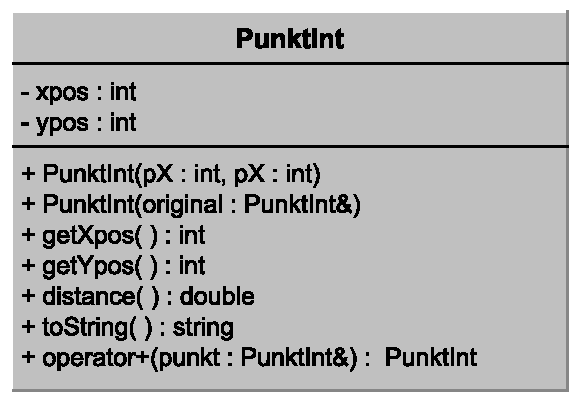
\includegraphics[keepaspectratio,scale=0.7]{punktint-uml.pdf}
\end{center}

\begin{enumerate}
	\item Erstellen Sie zu obigem Klassendiagramm die Klassendefinition von \code{PunktInt} in einer separaten Schnittstellendatei \code{PunktInt.h}.
	Achten Sie darauf, dass ein mehrfaches Einbinden von \code{PunktInt.h} verhindert wird.
	\item Implementieren Sie den ersten Konstruktor der Klasse \code{PunktInt}. Dieser nimmt zwei \code{int}-Zahlen entgegen, die die Koordinaten des Punktes festlegen.
	\item Implementieren Sie den Kopierkonstruktor. Verwenden Sie dafür den zuerst implementierten Konstruktor.
	\item Implementieren Sie die beiden Getter-Methoden \code{getXpos} und \code{getYpos}.
	\item Implementieren Sie die Methode \code{distance}, die die Entfernung des Punktes mit den Koordinaten $(\code{xpos}, \code{ypos})$ zum Ursprung $(0,0)$ berechnet.
	
	\textbf{Hinweis:} Die Wurzel einer Zahl kann mit der Methode \code{sqrt} aus der Bibliothek \code{cmath} berechnet werden.
	\item Implementieren Sie die Methode \code{toString}, die für einen Punkt $(x,y)$ die Stringdarstellung \code{(x,y)} zurückgibt.
	
	\textbf{Hinweis:} Die Methode \code{std::to\_string} wandelt Zahlen in Strings um.
	\item Überladen Sie den Operator \code{+}. Die Summe zweier Punkte $(a,b)$ und $(x,y)$ ist dabei ein neuer Punkt mit den Koordinaten $(a+x,b+y)$.
	\item Ergänzen Sie jede Methode um das Schlüsselwort \code{const}, wo dies sinnvoll erscheint.
	\item Angenommen, Sie möchten nun eine Klasse \code{PunktDouble} erstellen, die dieselbe Funktionalität wie \code{PunktInt} bereitstellt, aber Punkte mit Koordinaten vom Typ \code{double} realisiert.
	An welchen Stellen unterscheidet sich diese Klasse von der Klasse \code{PunktInt}? Wie sieht es aus, wenn Sie eine Klasse \code{PunktFloat} realisieren?
\end{enumerate}
\end{document}